\documentclass{theozettel}

%%%%%%%%%%%%%%%%%%%%%%%%%%%%%%%%%%%%%%%%%%%%%%%%%%%%%%%%%%%%%%%%%%%%%%%%%%%%%%%%%%%%%%%%%%%%%%%%%%%%%%%%%%%%%%
% page geometry
%%%%%%%%%%%%%%%%%%%%%%%%%%%%%%%%%%%%%%%%%%%%%%%%%%%%%%%%%%%%%%%%%%%%%%%%%%%%%%%%%%%%%%%%%%%%%%%%%%%%%%%%%%%%%%
\geometry{
	left=20mm,
	right=20mm,
	top=25mm,
	bottom=20mm
}
%%%%%%%%%%%%%%%%%%%%%%%%%%%%%%%%%%%%%%%%%%%%%%%%%%%%%%%%%%%%%%%%%%%%%%%%%%%%%%%%%%%%%%%%%%%%%%%%%%%%%%%%%%%%%%

\pgfplotsset{compat=1.16}

\usepackage{dsfont}

\theoI{2}

\renewcommand{\epsilon}{\varepsilon}

\begin{document}
\punkteIV{2.1}{2.2}{2.3}{2.4}

\section*{Aufgabe 2.1}
\begin{enumerate}[(a)]
	\item 	Wir betrachten $\vec{x} = (x_{1}, 0, 0)$ und $\vec{y}=(y_{1},y_{2},0)$ mit $x_{1}, y_{1}, y_{2} > 0$. Dann gilt für $\vec{z} = \vec{x} \times \vec{y}$:
			\[
				z_{i} = \sum_{j=1}^{3}\sum_{k=1}^{3} \epsilon^{ijk}x_{j}y_{j} \stackrel{x_{2}=x_{3}=0}{=} \underbrace{\epsilon^{i11}}_{= 0}x_{1}y_{1} + \epsilon^{i12}x_{1}y_{2} + \epsilon^{i13}x_{1}\underbrace{y_{3}}_{= 0} = \epsilon^{i12}x_{1}y_{2}.
			\]
			Mit der Definition des Levi-Civita-Symbols erhalten wir also:
			\[
				z_{1} = z_{2} = 0, \ \ \ \ \  z_{3} = x_{1}y_{2}.
			\]
			$\vec{x}$ und $\vec{y}$ liegen in der Ebene gegeben durch alle $\vec{a}$ mit $a_{3} = 0$ und der Winkel von $\theta$ zwischen $\vec{x}$ und $\vec{y}$ ist genau der Winkel zwischen $\vec{y}$ und der ersten Koordinatenachse. Dies wird an folgender Abbildung klar:
			\begin{figure}[h]
			\centering
			\begin{tikzpicture}
				\draw[->] (-0.5,0) -- (6,0);
				\draw[->] (0,-0.5) -- (0,4);
				
				\draw[->, thick, blue] (0,0) -- (5.3,0);
				\node at (4.5,0) [label=below:\textcolor{blue}{$\vec{x}$}] {};
				
				\draw[->, thick, red] (0,0) -- (4,3);
				\node at (2,1.5) [label=left:\textcolor{red}{$\vec{y}$}] {};
				
				\draw[thick, red] (0,0) -- (4,0);
				\node at (2,0) [label=below:\textcolor{red}{$y_{1}$}] {};
				
				\draw[thick, red] (4,0) -- (4,3);
				\node at (4,1.5) [label=right:\textcolor{red}{$y_{2}$}] {};
			\end{tikzpicture}
			\end{figure}
			
			Dann sehen wir geometrisch ein:
			\[
				\sin(\theta) = \frac{y_{2}}{\qty|\vec{y}|}
			\]
			Woraus wir direkt folgern:
			\[
				\qty|\vec{z}| = x_{1}y_{2} =x_{1} \cdot y_{2} \cdot \frac{\qty|\vec{y}|}{\qty|\vec{y}|} = \qty|x| \cdot \qty|y| \cdot \sin(\theta).
			\]
			Ferner folgt $\vec{z} \perp \vec{x}$ und $\vec{z} \perp \vec{y}$ durch:
			\begin{align*}
				\vec{z} \cdot \vec{x} &= x_{1}z_{1} + x_{2}z_{2} + x_{3}z_{3} = x_{1} \cdot 0 + 0 \cdot 0 + 0 \cdot z_{3} = 0, \\
				\vec{z} \cdot \vec{y} &= y_{1}z_{1} + y_{2}z_{2} + y_{3}z_{3} = y_{1} \cdot 0 + y_{2} \cdot 0 + 0 \cdot z_{3} = 0.
			\end{align*}
			
	\item 	Es ist $\epsilon^{ijk} = 0$ genau dann wenn zwei Indizes gleich sind. In diesem Fall ist die Antisymmetrie klar. Nun seien $i,j,k$ also verschieden. Dann wird die Antisymmetrie klar, durch aufzählen aller möglichen Fälle:
			\begin{align*}
				\epsilon^{123} = 1 &&& \longleftrightarrow &&& \epsilon^{213} = -1 \\
				&&& \longleftrightarrow &&& \epsilon^{321} = -1 \\
				&&& \longleftrightarrow &&& \epsilon^{132} = -1 \\
				\epsilon^{312} = 1 &&& \longleftrightarrow &&& \epsilon^{132} = -1 \\
				&&& \longleftrightarrow &&& \epsilon^{213} = -1 \\
				&&& \longleftrightarrow &&& \epsilon^{321} = -1 \\
				\epsilon^{231} = 1 &&& \longleftrightarrow &&& \epsilon^{321} = -1 \\
				&&& \longleftrightarrow &&& \epsilon^{132} = -1 \\
				&&& \longleftrightarrow &&& \epsilon^{213} = -1 \\
			\end{align*}
			Wir folgern:
			\begin{align*}
				\vec{x} \cdot (\vec{x} \times \vec{y}) &= \mqty(x_{1} \\ x_{2} \\ x_{3}) \cdot \mqty( \sum_{j=1}^{3}\sum_{k=1}^{3} \epsilon^{1jk}x_{j}y_{k}2 \\ \sum_{j=1}^{3}\sum_{k=1}^{3} \epsilon^{2jk}x_{j}y_{k} \\ \sum_{j=1}^{3}\sum_{k=1}^{3} \epsilon^{3jk}x_{j}y_{k}) = \mqty(x_{1} \\ x_{2} \\ x_{3}) \cdot \mqty( \epsilon^{123}x_{2}y_{3} + \epsilon^{132}x_{3}y_{2} \\ \epsilon^{213}x_{1}y_{3} + \epsilon^{231}x_{3}y_{1} \\ \epsilon^{312}x_{1}y_{2} + \epsilon^{321}x_{2}y_{1} ) \\		
				&= x_{1}\epsilon^{123}x_{2}y_{3} +x_{2}\epsilon^{213}x_{1}y_{3} + x_{1}\epsilon^{132}x_{3}y_{2} + x_{3}\epsilon^{312}x_{1}y_{2} + x_{2}\epsilon^{231}x_{3}y_{1} + x_{3}\epsilon^{321}x_{2}y_{1} \\
				&= 	\epsilon^{123}x_{1}x_{2}y_{3} - \epsilon^{123}x_{1}x_{2}y_{3} + \epsilon^{132}x_{1}x_{3}y_{2} -\epsilon^{132}x_{1}x_{3}y_{2} + \epsilon^{231}x_{2}x_{3}y_{1} - \epsilon^{231}x_{2}x_{3}y_{1} \\ &= 0.
			\end{align*}
			Vollkommen analog rechnen wir $\vec{y} \cdot (\vec{x} \times \vec{y})$. 
\end{enumerate}


\newpage
\subsection*{Aufgabe 2.2}Die periodische Bewegung eines Teilchens sei beschrieben durch
	\begin{align*}	
	\vec{x}\left(t\right) =
	\begin{pmatrix}
	x_1\left(t\right)\\
	x_2\left(t\right)\\
	\end{pmatrix}
	= R \cos\left(\omega t \right)
	\begin{pmatrix}
	1\\
	\sin\left(\omega t\right)\\
	\end{pmatrix}
	\end{align*}
	\subsubsection*{a)}Berechnen Sie die Geschwindigkeit $\vec{v}\left(t\right)$ und die Beschleunigung $\vec{a}\left(t\right)$ Des Teilchens.\\\\
	Um die Geschwindigkeit und die Beschleunigung zu berechnen, leiten wir $\vec{x}\left(t\right)$ nach der Zeit ($t$) ab.\\
	Aus "Ubersichtsgr"unden werden wir dies Komponentenwei"se machen.\\\\
	Zuerst f"ur die Geschwindigkeit:
	\begin{align*}
	x_1\left(t\right) &= R \cos\left(\omega t\right)\\
	 v_1\left(t\right) =\dot{x_1}\left(t\right) &= - R \omega \sin\left(\omega t\right)\\\\	 
	 x_2\left(t\right) &= R \cos\left(\omega t\right)\sin\left(\omega t\right)\\
	 v_2\left(t\right) =\dot{x_2}\left(t\right) &=  R \omega \left[\cos^2\left(\omega t\right) - \sin^2\left(\omega t\right)\right]\\
	\end{align*}
	Zusammengesetzt ergibt dies:
	\begin{align*}	
	\vec{v}\left(t\right) =
	\begin{pmatrix}
	- R \omega \sin\left(\omega t\right)\\
	R \omega \left[\cos^2\left(\omega t\right) - \sin^2\left(\omega t\right)\right]\\
	\end{pmatrix}
	= R\omega
	\begin{pmatrix}
	-\sin\left(\omega t\right)\\
	\left[\cos^2\left(\omega t\right) - \sin^2\left(\omega t\right)\right]\\
	\end{pmatrix}
	\end{align*}
	
	Die Beschleunigung ist die Ableitung der Geschwindigkeit nach der Zeit.\\
	In Komponentenschreibwei"se:
	\begin{align*}
	v_1\left(t\right) &=  - R \omega \sin\left(\omega t\right)\\
	 a_1\left(t\right) =\dot{v_1}\left(t\right) &= - R \omega^2 \cos\left(\omega t\right)\\\\	 
	 v_2\left(t\right) &= R \omega \left[\cos^2\left(\omega t\right) - \sin^2\left(\omega t\right)\right]\\
	 a_2\left(t\right) =\dot{v_2}\left(t\right) &= -4 R \omega^2  \cos\left(\omega t\right) \sin\left(\omega t\right)\\
	\end{align*}
	Zusammengesetzt ergibt dies:
	\begin{align*}	
	\vec{a}\left(t\right) =
	\begin{pmatrix}
	- R \omega^2 \cos\left(\omega t\right)\\
	-4 R \omega^2  \cos\left(\omega t\right) \sin\left(\omega t\right)\\
	\end{pmatrix}
	= -R\omega^2
	\begin{pmatrix}
	 \cos\left(\omega t\right)\\
	4 \cos\left(\omega t\right) \sin\left(\omega t\right)\\
	\end{pmatrix}
	\end{align*}
	\subsubsection*{b)}Fertigen Sie eine Skizze der Teilchenbahn an (Raumkurve in zwei Dimensionen). Tragen Sie dazu auf den Koordinatenachsen die Werte $x_1 \left( t \right)/R$ und $x_2 \left( t \right) /R$ auf. beachten Sie, dass das Teilchen auch eine Auslenkung in $x_2$ -Richtung besitzt. Identifizieren Sie die Positionen $\vec{x} \left( t_0 \right) $ f"ur $ \omega t_0 = 0, \pi /2, \pi, 3\pi /2$. Achten Sie auf eine korrekte Beschriftung der Achsen.\\\\
	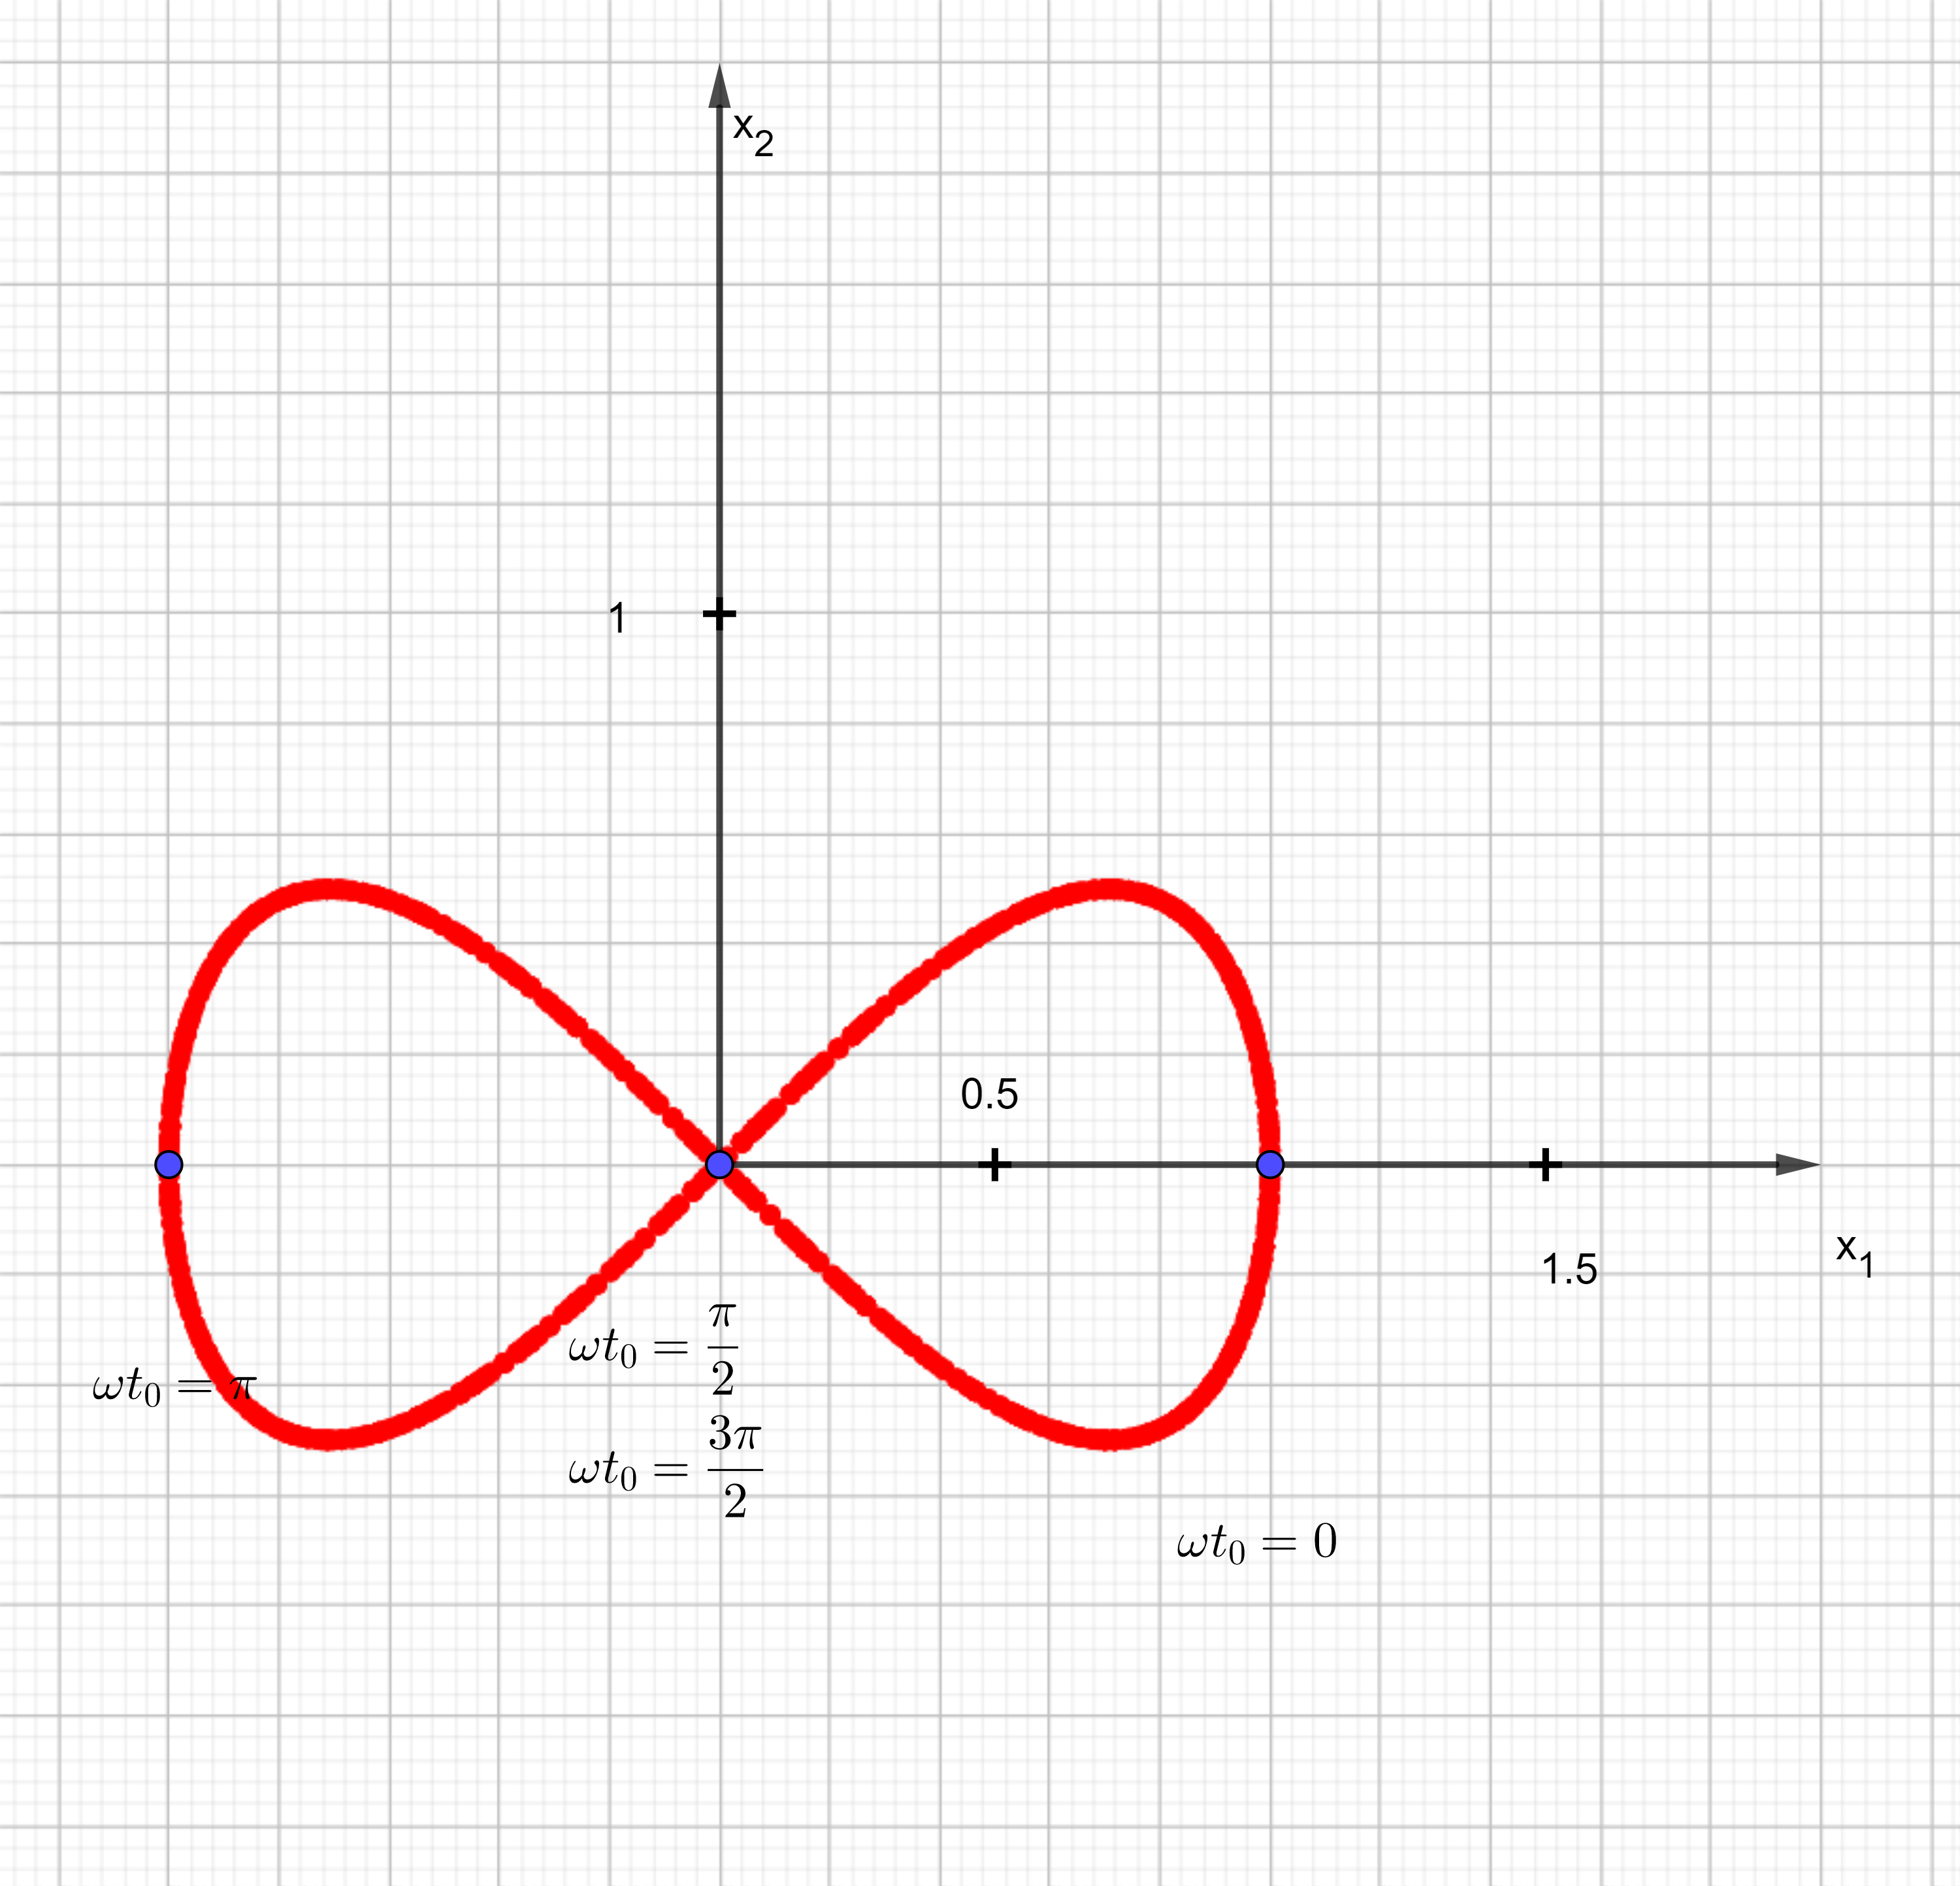
\includegraphics[scale=2.4]{A2-2b.png}
	\subsubsection*{c)}Tragen Sie in die obige Skizze die EInheitsverktoren $\vec{v}\left(t_0\right)/|\vec{v}\left(t_0\right)|$ und $\vec{a}\left(t_0\right)/|\vec{a}\left(t_0\right)|$ am Punkt $\vec{x}\left(t_0\right) = R \left(\begin{smallmatrix}1\\0\end{smallmatrix}\right)$ ein.\\\\
	$\vec{v}_n$ = $\vec{v}\left(t_0\right)/|\vec{v}\left(t_0\right)|$ und  $\vec{a}_n$ = $\vec{a}\left(t_0\right)/|\vec{a}\left(t_0\right)|$\\
	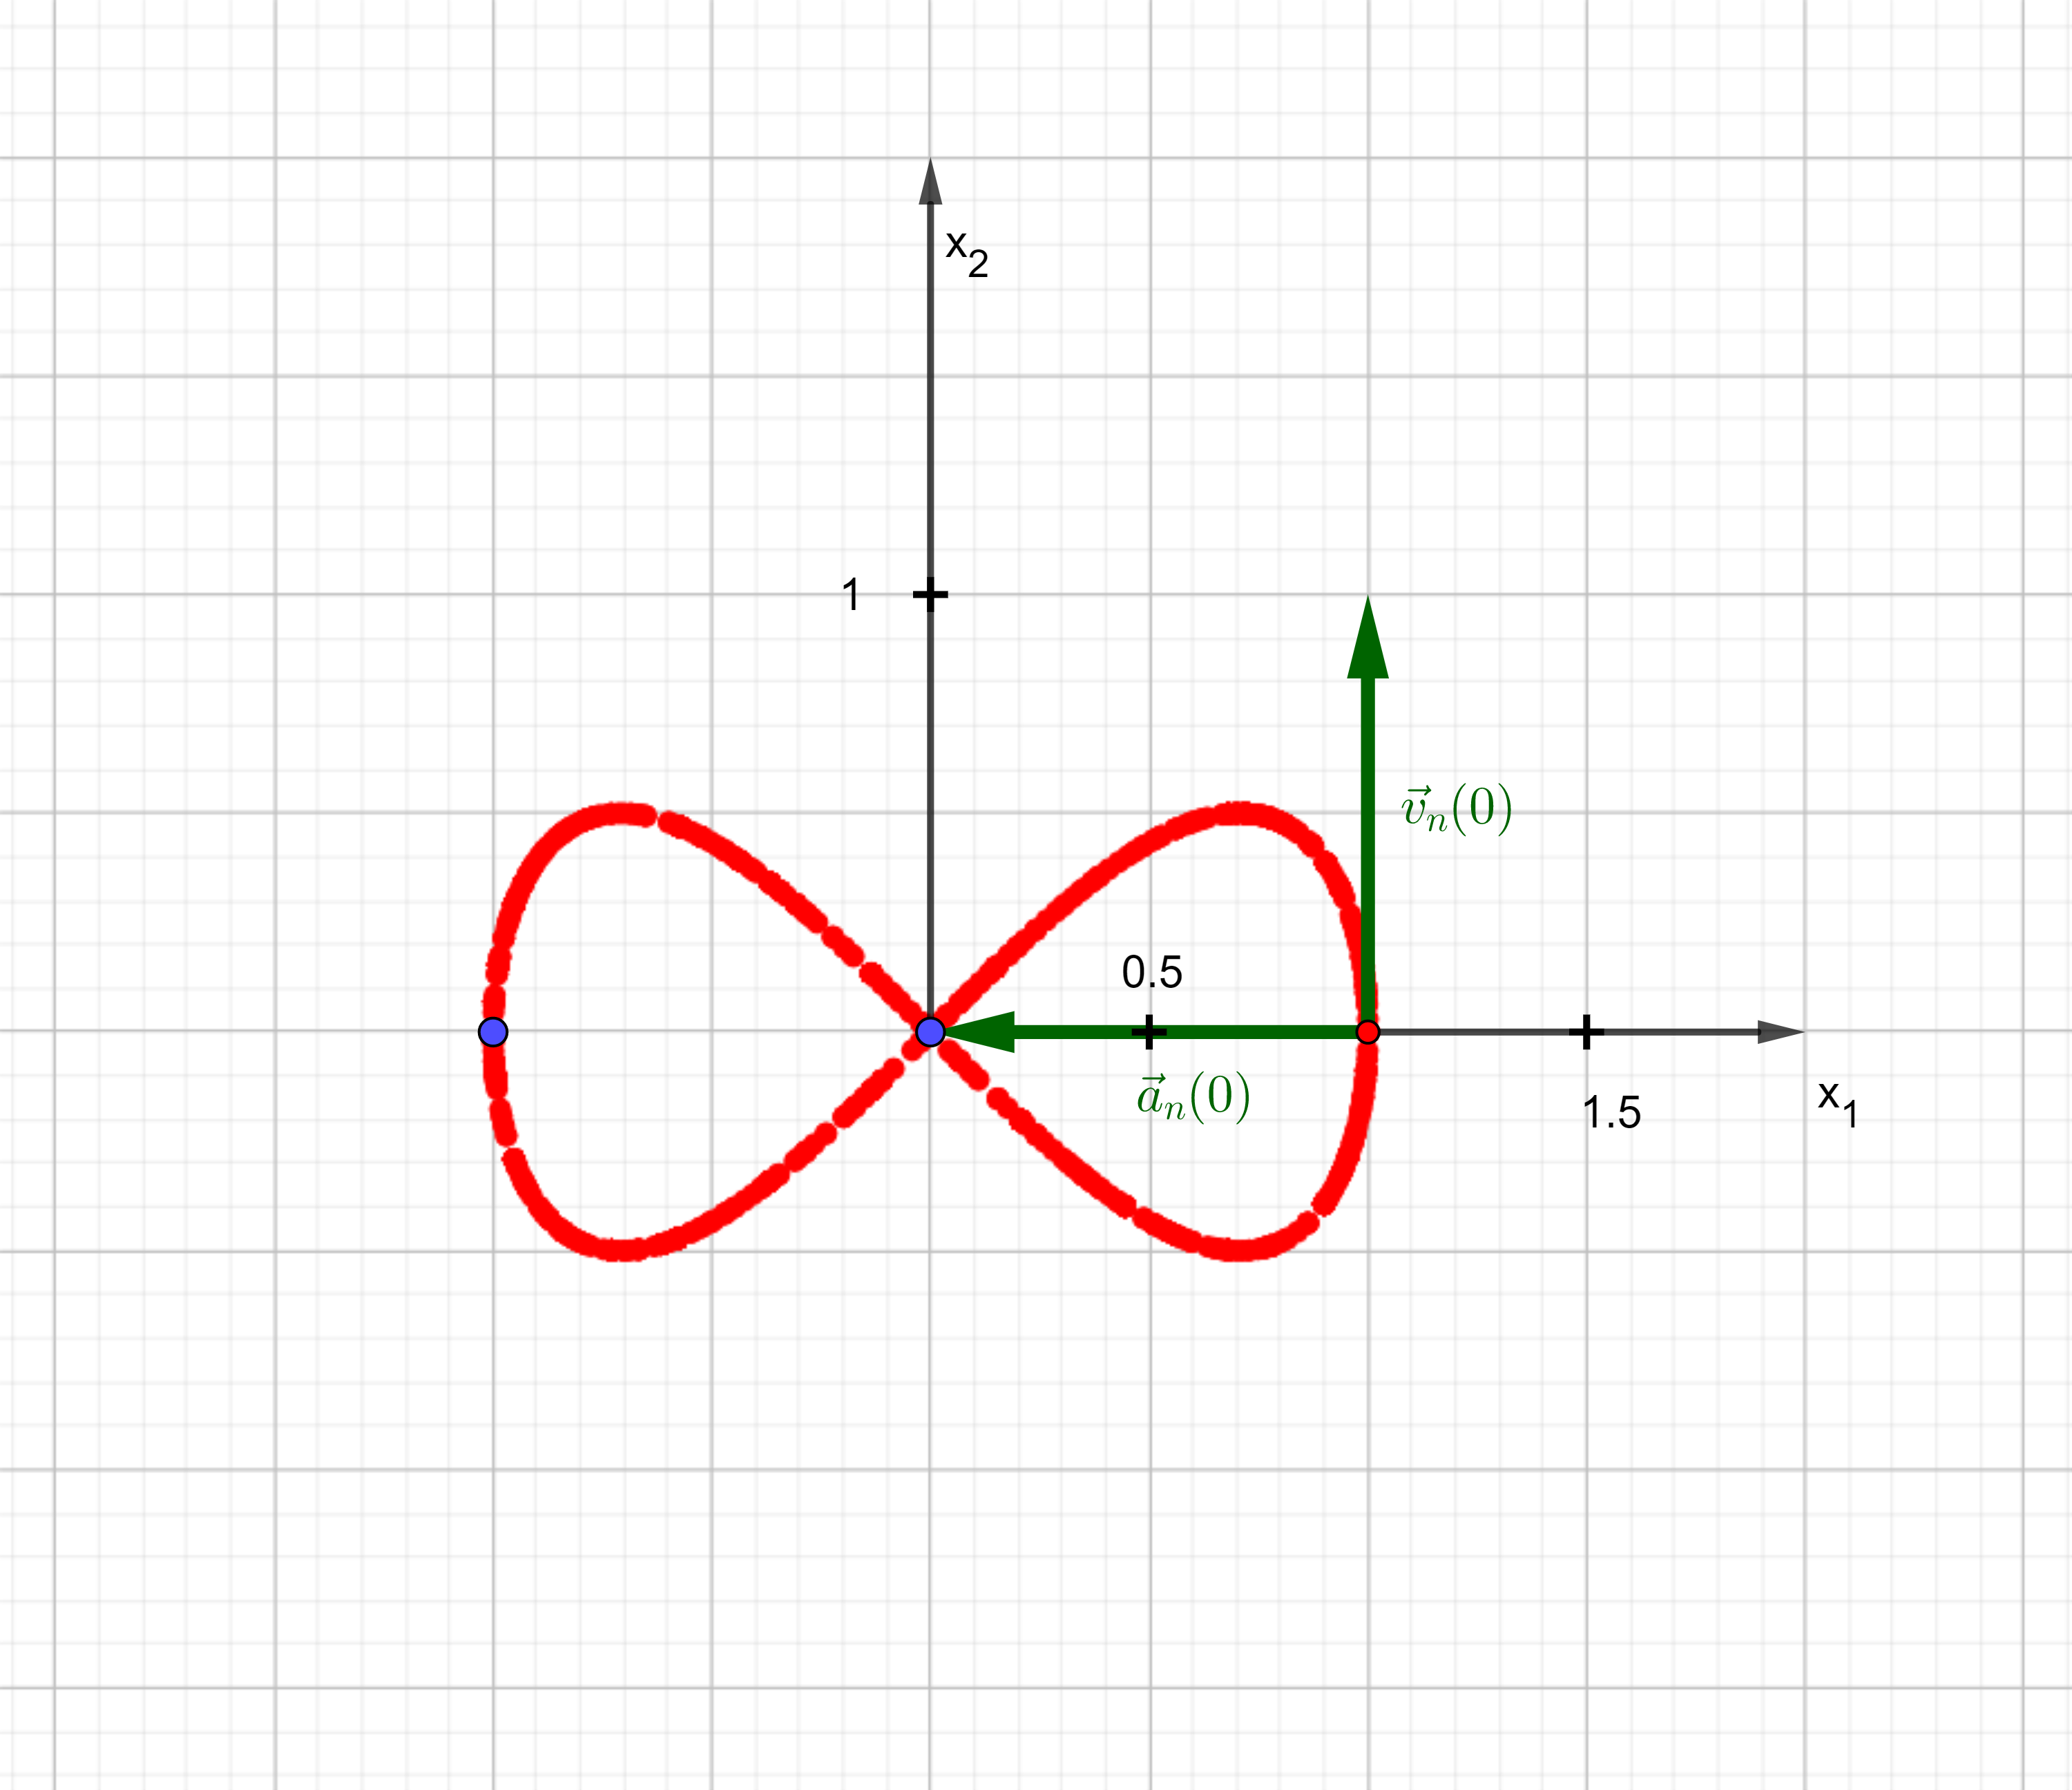
\includegraphics[scale=2.4]{A2-2c.png}


\newpage
\section*{Aufgabe 2.3}

a)

Der Geschwindigkeitsvektor ergibt sich aus der Ableitung des Positionsvektors:

$$
\vec{x}(t) = \begin{pmatrix}
R cos(\omega t) \\
R sin(\omega t) \\
v_0 t
\end{pmatrix}
$$

$$
\vec{v	}(t) = \dot{vec{x}}(t) = \begin{pmatrix}
- R \omega sin(\omega t) \\
R \omega cos(\omega t) \\
v_0
\end{pmatrix}
$$

Die Bogenlänge berechnet sich wie folgt:

$$
s(t) =  \int_{t_0}^{t} d t' | \vec{v}(t') | = \int_{t_0}^{t} d t' \sqrt{\vec{v}(t')^{2}} = \int_{0}^{t} d t' \sqrt{R^{2}\omega^{2} ((-sin(\omega t'))^{2} + cos(\omega t')^{2} + v_0^{2}} = \sqrt{R^{2} \omega^{2} + v_0^{2}} t
$$

Man beachte hierbei, dass die Integrationskonstante tatsächlich $0$ ist, da $s(t_0 = 0) = 0$ angenommen wurde.

Die Formel kann umgestellt werden zu:

$$
t(s) = \frac{s}{\sqrt{R^{2} \omega^{2} + v_0^{2}}}
$$

Der Tangentenvektor entspricht dem auf $1$ normierten Geschwindigkeitsvektor:

$$
\vec{T}(s) = \frac{\vec{v}(t(s))}{|\vec{v}(t(s))|} = \frac{1}{\sqrt{R^{2} \omega^{2} + v_0^{2}}} \begin{pmatrix}
- R \omega sin(\frac{\omega s}{\sqrt{R^{2} \omega^{2} + v_0^{2}}}) \\
R \omega cos(\frac{\omega s}{\sqrt{R^{2} \omega^{2} + v_0^{2}}}) \\
v_0
\end{pmatrix}
$$

Für den Krümmungsradius gilt:

$$
\rho = \frac{1}{|\frac{d\vec{T}}{ds}|} = \frac{1}{|\begin{pmatrix}
\frac{- R \omega^{2}}{\sqrt{R^{2} \omega^{2} + v_0^{2}}}cos(\frac{\omega s}{\sqrt{R^{2} \omega^{2} + v_0^{2}}}) \\
\frac{- R \omega^{2}}{\sqrt{R^{2} \omega^{2} + v_0^{2}}}sin(\frac{\omega s}{\sqrt{R^{2} \omega^{2} + v_0^{2}}}) \\
0
\end{pmatrix} |} = \frac{1}{\frac{- R \omega^{2}}{\sqrt{R^{2} \omega^{2} + v_0^{2}}}}
$$

Der Normalenvektor ergibt sich wie folgt:

$$
\vec{N}(s) = \rho \frac{d\vec{T}}{ds} =\begin{pmatrix}
-cos(\frac{\omega s}{\sqrt{R^{2} \omega^{2} + v_0^{2}}}) \\
-sin(\frac{\omega s}{\sqrt{R^{2} \omega^{2} + v_0^{2}}}) \\
0
\end{pmatrix} 
$$

Der Binormalenvektor berechnet sich wie folgt:

\begin{align}
\vec{B}(s) &= \vec{T}(s) \times \vec{N}(s) \\&= \frac{1}{\sqrt{R^{2} \omega^{2} + v_0^{2}}} \begin{pmatrix}
R \omega cos(\omega t(s)) 0 - v_0 (-sin(\omega t(s))) \\
v_0 -cos(\omega t(s)) - 0 (-R \omega sin(\omega t(s)) \\
-R \omega sin(\omega t(s) (-sin(\omega t(s)))  - R \omega \cos(\omega t(s)) (-cos(\omega t(s)))
\end{pmatrix} \\ &= \frac{1}{\sqrt{R^{2} \omega^{2} + v_0^{2}}} \begin{pmatrix}
v_0 (-sin(\omega \frac{s}{\sqrt{R^{2} \omega^{2} + v_0^{2}}})) \\
v_0 (-cos(\omega \frac{s}{\sqrt{R^{2} \omega^{2} + v_0^{2}}})) \\
R \omega
\end{pmatrix}
\end{align}
b)

Aufgrund der alternativen Definition des Vektorprodukts muss gelten, dass $\vec{B}(s) \perp \vec{T}(s)$ und $\vec{B}(s) \perp \vec{N}(s)$. Dass $\vec{B}(s) \perp \vec{N}(s)$ gilt, kann dadurch gezeigt werden, dass das Skalarprodukt $0$ ist:

\begin{align}
\vec{T}(s) \cdot \vec{N}(s) &= \frac{1}{\sqrt{R^{2} \omega^{2} + v_0^{2}}}
((- R \omega sin(\frac{\omega s}{\sqrt{R^{2} \omega^{2} + v_0^{2}}})) (-cos(\frac{\omega s}{\sqrt{R^{2} \omega^{2} + v_0^{2}}})) \\&+ (R \omega cos(\frac{\omega s}{\sqrt{R^{2} \omega^{2} + v_0^2}})) (-sin(\frac{\omega s}{\sqrt{R^{2} \omega^{2}
+ v_0^{2}}})) + 0 v_0 = 0
\end{align}




\newpage
\subsection*{Aufgabe 2.4} Zeigen Sie durch Integration, dass
\begin{align*}
\int{\frac{dx}{\sqrt{ax^2+2bx+c}}}=- \frac{1}{\sqrt{-a}}\arcsin{\frac{ax+b}{\sqrt{b^2-ac}}} \text{, falls $a<0$ und $b^2 -ac>0$.}
\end{align*}\\
Zuerst betrachten wir nur den Term unter der Wurzel:
\begin{align*}
ax^2+2bx+c&=a\left(x^2+\frac{2b}{a}x+\frac{c}{a}\right)\\
\text{Nun erg"anzen wir quadratisch:}\\
&=a\left(x^2+\frac{2b}{a}x+\left(\frac{b}{a}\right)^2-\left(\frac{b}{a}\right)^2+\frac{c}{a}\right)\\
\text{Nun wenden wir die 1. binomische Formel an:}\\
&= a\left(\left( x+\frac{b}{a} \right)^2 - \left(\frac{b}{a}\right)^2+\frac{c}{a}\right)\\
&= a\left(\left( x+\frac{b}{a} \right)^2- (\frac{b^2+ac}{a^2}\right)\\
\end{align*}
\begin{align*}
\text{Nun klammern wir ein \glqq -\grqq aus und stellen die Gleichung ein bisschen um:}\\
= -a\left(\frac{b^2-ac}{a^2} - \left( x+\frac{b}{a} \right)^2 \right)\\
\end{align*}
Nach dieser Umformung werden wir das Integral mehrmals substituieren.
\begin{align*}
\int{\frac{dx}{\sqrt{-a\left(\frac{b^2-ac}{a^2} - \left( x+\frac{b}{a} \right)^2 \right)}}}\\
\end{align*} 
\begin{align*}
\text{Nun substituieren wir mit $y= x + \frac{b}{a}$, gleichzeitig setzen wir $y_0 = \sqrt{\frac{b^2-ac}{a^2}}$}\\
\end{align*}
\begin{align*}
\frac{dy}{dx} = 1 \ \Rightarrow dy=dx
\end{align*} 
Daraus ergibt sich:
\begin{align*}
\int{\frac{dy}{\sqrt{-a\left(y_0^2-y^2\right)}}}=\frac{1}{\sqrt{-a}}\int{\frac{dy}{\sqrt{y_0^2-y^2}}}
\end{align*}
Als n"achstes substituieren wir $y$ mit $y= y_0 \sin{\phi}$:
\begin{align*}
\frac{dy}{d\phi}=y_0 \cos{\phi} \ \Rightarrow dy = d\phi \ y_0 \cos{\phi}
\end{align*}
Mit dieser Substitution ergibt sich:
\begin{align*}
\frac{1}{\sqrt{-a}}\int{\frac{d\phi \ y_0 \cos{\phi}}{\sqrt{y_0^2- \left(y_0 \sin{\phi}\right)^2}}}&= \frac{1}{\sqrt{-a}}\int{\frac{d\phi \ y_0 \cos{\phi}}{\sqrt{y_0^2\left(1- \sin^2{\phi}\right)}}}\\
&=\frac{1}{\sqrt{-a}}\int{\frac{d\phi \ y_0 \cos{\phi}}{\sqrt{y_0^2\cos^2{\phi}}}}\\
&=\frac{1}{\sqrt{-a}}\int{\frac{d\phi \ y_0 \cos{\phi}}{y_0\cos{\phi}}}\\
&=\frac{1}{\sqrt{-a}}\int{d\phi\frac{y_0\cos{\phi}}{y_0\cos{\phi}}}\\
&=\frac{1}{\sqrt{-a}}\int{1 \ d\phi}\\
&= \frac{1}{\sqrt{-a}} \ \phi
\end{align*}
Nun m"ussen wir nur noch die Substitutionen nach $\phi$ aufl"osen und f"ur $\phi$ einsetzen:
\begin{align*}
 y=y_0 \sin{\phi} &\Rightarrow \sin{\phi}=\frac{y}{y_0}\\
 &\Rightarrow \phi = \arcsin{\frac{y}{y_0}}
\end{align*}
Mit $y= x + \frac{b}{a}$ und $y_0 = \sqrt{\frac{b^2-ac}{a^2}}$ ergibt sich f"ur $\phi$:
\begin{align*}
\phi &= \arcsin{\frac{x + \frac{b}{a}}{\sqrt{\frac{b^2-ac}{a^2}}}}\\
&= \arcsin{\frac{x + \frac{b}{a}}{\sqrt{b^2-ac}\cdot\sqrt{\frac{1}{a^2}}}}\\
&= \arcsin{\frac{\sqrt{a^2}\left(x+\frac{b}{a}\right)}{\sqrt{b^2-ac}}}
\end{align*}
Wir betrachten nun die Werte unter den Wurzeln:\\
Als Konstante vor dem Integrierten haben wir $\frac{1}{\sqrt{-a}}$, somit muss $a<0$ sein.\\
Auch muss $b^2>ac$ gelten, da sonst der Nenner im $\arcsin$ nicht l"osbar w"are.\\\\
Durch den Fakt, dass $a<0$, kann $\sqrt{a^2}$ als $-a$ interpretiert werden.\\
Damit ergibt sich f"ur $\phi$:
\begin{align*}
\phi= \arcsin{\frac{-a\left(x+\frac{b}{a}\right)}{\sqrt{b^2-ac}}}\\
\end{align*} 
F"ur $\arcsin$ gilt: $\arcsin\left(-x\right)=-\arcsin\left(x\right)$.\\
Somit gilt f"ur $\phi$:
\begin{align*}
\phi &= -\arcsin{\frac{a \left(x+\frac{b}{a}\right)}{\sqrt{b^2-ac}}}\\
&= - \arcsin{\frac{ax+b}{\sqrt{b^2-ac}}}
\end{align*} 
Setzen wir dies nun f"ur $\phi$ in $\frac{1}{\sqrt{-a}}\phi$ ein, so ergibt dies, falls $a<0$ und $b^2>ac$:
\begin{align*}
\int{\frac{dx}{\sqrt{ax^2+2bx+c}}}=- \frac{1}{\sqrt{-a}}\arcsin{\frac{ax+b}{\sqrt{b^2-ac}}}
\end{align*}
Dies entspricht der zu beweisenden Integration.\qquad\qquad\qquad\qquad\qquad\qquad\qquad\qquad\qquad\qquad\qquad\qquad $\blacksquare$

\end{document}